\documentclass[ignorenonframetext,ucs]{beamer}

\usepackage[ngerman]{babel}
\usepackage{ucs}
\usepackage[utf8x]{inputenc}
\usepackage[T1]{fontenc}
\usepackage{relsize}
\usepackage{lmodern}

\PreloadUnicodePage{0}

%\usepackage[colorlinks]{hyperref}
\newcommand\refurl[2]{#2\footnote{\url{#1}}}

\usepackage{graphicx}
\definecolor{darkgreen}{rgb}{0,0.5,0}
\usetheme[compress]{Berlin}

\title{Unter~dem~Radar~— Das~Zensusgesetz~2011}
\subtitle{All~Your~Database Are~Belong To~Us}
\author{Oliver~„Unicorn“~Knapp \and Tim~„Scytale“~Weber}
\institute{
	Chaos~Computer~Club~e.V. % \and
%	oqlt~e.V. \and
%	RaumZeitLabor~Mannheim
}
\date{22.~Mai~2010\\SIGINT~2010, Köln}

\begin{document}

\frame{\titlepage}

\section{Einführung}

\subsection{Die Referenten}

\subsection{Der Zensus, das unbekannte Wesen}

\begin{frame}{Was ist ein Zensus?}\begin{itemize}
\item Volkszählung, Zensus, Census
\item mehr als nur Zählen
\item Makrozensus: alle werden gezählt
\item Mikrozensus: repräsentative Stichproben
\item Durchführungsarten:\begin{itemize}
	\item „klassischer“ Zensus: Umfragebögen
	\item Registerzensus: keine Umfragen, sondern Melderegister
	\item registergestützter Zensus: Mischform;\\Melderegister ergänzt durch Umfragen
\end{itemize}
\end{itemize}\end{frame}

\begin{frame}{Warum das Ganze?}\begin{itemize}
\item Bevölkerungszusammensetzung und -verteilung
\item Planung (Wohnungsbau, Infrastruktur, …)
\item Finanzierung (Steuerschätzung, Länderfinanzausgleich,\\kommunale Haushalte, …)
\item Bildungsniveau, Ausländeranteil, Religionszugehörigkeit, Familienstruktur, …)
\end{itemize}\end{frame}

\subsection{Geschichte der Volkszählungen}

\begin{frame}{Im Nationalsozialismus}\begin{itemize}
\item 1933, 1939; Volks-, Berufs-, Betriebszählungen
\item Erfassung von „Glaubens-“ und „Geltungsjuden“\\sowie „Mischlingen“
\item Name, Geburtsname, Religion, Muttersprache,\\Volkszugehörigkeit, Beruf
\item Verwandschaftsbeziehung
\end{itemize}\end{frame}

\begin{frame}{In der DDR}\begin{itemize}
\item 1950 und 1964 Volks- und Berufszählungen
\item 1971 und 1981 Volks-, Berufs-, Wohnraum-\\und Gebäudezählungen
\item Ergebnisse aus politischen Gründen\\teilweise nicht veröffentlicht
\end{itemize}\end{frame}

\begin{frame}{In der Bundesrepublik}\begin{itemize}
\item 1961 und 1970 Volks- Berufs- und Arbeitsstättenzählungen
\item 1950 und 1987 Volks-, Berufs-, Gebäude-, Wohnungs-\\und Arbeitsstättenzählungen
\item Volkszählung egtl. für 1981 geplant\begin{itemize}
	\item Finanzierungsstreit, Gesetz erst 1982 verabschiedet
	\item Zähltermin daher 1983
	\item Verfassungsklage, Änderungsbedarf
	\item verschoben bis 1987
\end{itemize}
\end{itemize}\end{frame}

\subsection{Die Volkszählung 1983/87}

\subsection{Volkszählungen nach der Wiedervereinigung}

\begin{frame}{Deutsche Volkszählung 1991}\begin{itemize}
\item angedacht wegen Wiedervereinigung
\item nicht durchgeführt:\begin{itemize}
	\item finanzielle Gründe
	\item Ablehnung in Politik und Bevölkerung
\end{itemize}
\end{itemize}\end{frame}

\begin{frame}{EU-Zensusrunde 2000/2001}\begin{itemize}
\item ohne Schweden und Deutschland
\item deutsches Argument: Ablehnung bei Bevölkerung
\end{itemize}
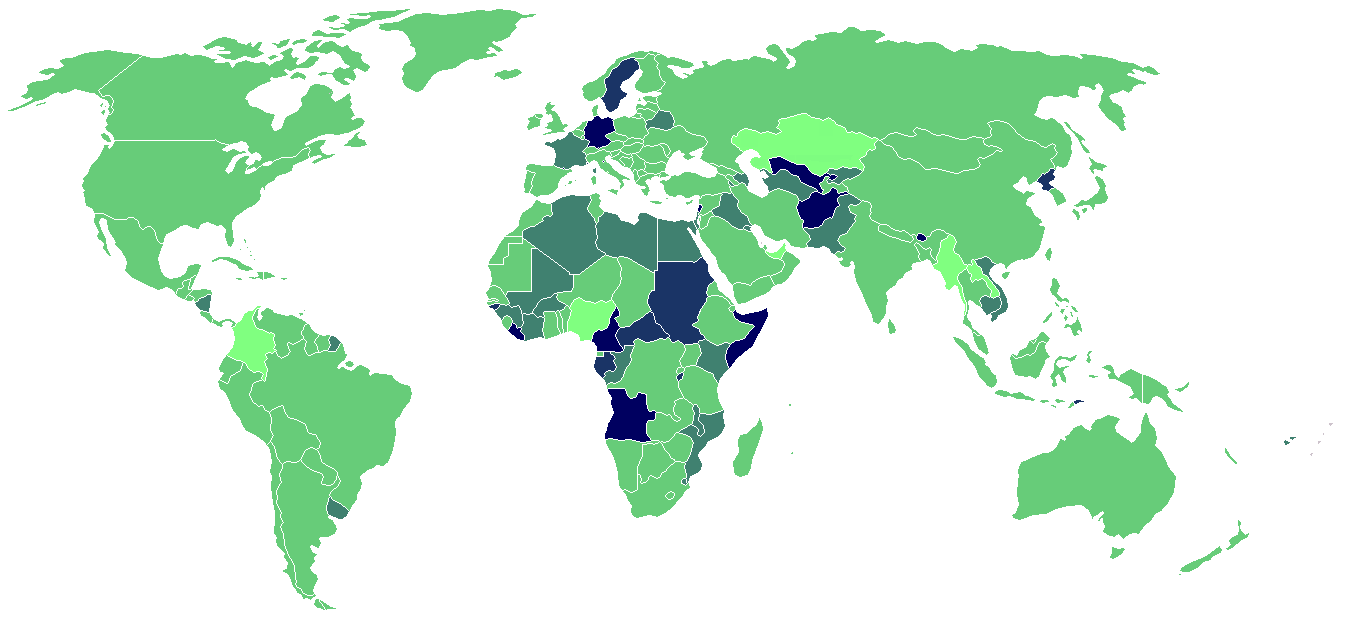
\includegraphics[height=4cm]{most-recent-census.png}
\end{frame}

\begin{frame}{Steuernummer 2007}\begin{itemize}
\item im Prinzip Registerzensus (Meldedaten)
\item bundesweite Personenkennziffer
\item Rückfluss an die Meldeämter
\item keine Verwendung für Statistik
\item Klage ist wohl vergessen worden
\end{itemize}\end{frame}

\section{Volkszählung 2011}

\subsection{Alles Gute kommt aus Brüssel}

\begin{frame}{Der EU-Beschluss}\begin{itemize}
\item registergestützter Zensus
\item Bundesregierung entscheidet August 2006:\\Deutschland macht mit
\end{itemize}\end{frame}

\subsection{Das Bundesgesetz}

\subsection{Umsetzung in den Ländern}

\begin{frame}{Anfrage Hessen}\begin{itemize}
\item mündliche Anhörung, bestritten durch Unicorn
\end{itemize}\end{frame}

\begin{frame}{Anfrage Thüringen}\begin{itemize}
\item schriftliche Anhörung (ergo: Text verfassen)
\end{itemize}\end{frame}

\section{Nächste Schritte}

\subsection{Liebesgrüße aus Karlsruhe}

\begin{frame}{Verfassungsklage}\begin{itemize}
\item Stichtag 16. Juli 2010 (1-Jahres-Frist)
\item bislang klagt noch niemand(!)
\item wer will?
\item Grüne haben 1983 protestiert,\\tragen das Gesetz jetzt mit
\item Linke sind eher dagegen
\item „die üblichen Verdächtigen“ müssen wohl ran
\end{itemize}\end{frame}

\begin{frame}{Argumente für die Klage}\begin{itemize}
\item informationelle Selbstbestimmung?
\item mehr als EU-Richtlinie (Religion)
\item bundeseinheitliche Personenkennziffer (Primärschlüssel)
\item fehlende Anonymisierung
\item umfassendes Personenprofil
\end{itemize}\end{frame}

\subsection{Tell a friend!}

\begin{frame}{Bevölkerung informieren}\begin{itemize}
\item Freunde, Familie, Aktivisten
\item Blogbeiträge
\item bei Presse und Rundfunk anfragen
\item Aktionen, Flyer, Aufkleber
\item you name it!
\end{itemize}\end{frame}

\end{document}
